\DomainHeader{Visualization}{8\%}

\begin{Objectives}
  \item Add a primvar to a mesh.
  \item Assign UsdPreviewSurface materials.
  \item Bind materials to a mesh.
  \item Build a UsdPreviewSurface network that reads diffuse colors from a primvar.
\end{Objectives}

\begin{Resources}
  \item Learn OpenUSD: Setting the Stage; Scene Description Blueprints;
        Beyond the Basics
  \item User guide: Rendering With USD
  \item OpenUSD glossary: Gprim
  \item OpenUSD API: UsdShadeMaterial; UsdShadeMaterialBindingAPI;
        UsdGeomSubset; UsdLux (LightAPI, ShadowAPI, ShapingAPI, DistantLight);
        Imageable Purpose
\end{Resources}

\CheatSheetTitle
\begin{itemize}[leftmargin=*]
  \item \textbf{UsdShade is scene description}: a \texttt{Material} prim is
        the public interface; \texttt{Shader} prims inside it form the
        network; attributes named \texttt{inputs:*}/\texttt{outputs:*}
        connect with \texttt{.connect}.\index{UsdShade}
  \item \textbf{Binding} is a relationship: \texttt{material:binding} on the
        gprim --- apply \texttt{MaterialBindingAPI} --- resolved via
        \texttt{ComputeBoundMaterial()}.\index{material binding}
  \item \textbf{UsdPreviewSurface} is the portable PBR shader ---
        \texttt{diffuseColor}, \texttt{roughness}, \texttt{metallic},
        \ldots\ --- paired with \texttt{UsdPrimvarReader} and
        \texttt{UsdUVTexture}.\index{UsdPreviewSurface}
  \item \textbf{Primvar-driven shading}: a reader node wired into
        \texttt{diffuseColor} lets \emph{one} material show per-prim colors
        --- instancing-friendly by design.
  \item \textbf{GeomSubset}: per-face material assignment without splitting
        the mesh --- \texttt{familyName = "materialBind"}, indices over
        faces.\index{GeomSubset}
  \item \textbf{purpose} tags subtrees: \texttt{default}, \texttt{proxy},
        \texttt{render}, \texttt{guide}; \texttt{visibility} inherits down
        namespace.\index{purpose}\index{visibility}
  \item \textbf{UsdLux}: lights are prims too; shared controls live in
        \texttt{LightAPI} (\texttt{inputs:intensity},
        \texttt{inputs:color}); \texttt{ShadowAPI}/\texttt{ShapingAPI}
        refine.\index{UsdLux}
\end{itemize}

\section{Core Concepts}

\subsection{One material, many looks: the primvar-driven network}\label{sec:vis-net}\objref{8.2, 8.4}
The exam's flagship task in this domain --- a UsdPreviewSurface whose diffuse
color comes from each mesh's \texttt{displayColor} primvar. Two plates, two
colors, \emph{one} material:

\begin{lstlisting}
#usda 1.0
(
    defaultPrim = "Scene"
    upAxis = "Y"
    metersPerUnit = 0.01
)
def Xform "Scene" {
    def Mesh "PlateA" (
        prepend apiSchemas = ["MaterialBindingAPI"]
    )
    {
        float3[] extent = [(-1, -1, 0), (1, 1, 0)]
        int[] faceVertexCounts = [4]
        int[] faceVertexIndices = [0, 1, 2, 3]
        point3f[] points = [(-1, -1, 0), (1, -1, 0), (1, 1, 0), (-1, 1, 0)]
        color3f[] primvars:displayColor = [(0.85, 0.35, 0.1)]
        rel material:binding = </Scene/Looks/Painted>
    }
    def Mesh "PlateB" (
        prepend apiSchemas = ["MaterialBindingAPI"]
    )
    {
        float3[] extent = [(-1, -1, 0), (1, 1, 0)]
        int[] faceVertexCounts = [4]
        int[] faceVertexIndices = [0, 1, 2, 3]
        point3f[] points = [(-1, -1, 0), (1, -1, 0), (1, 1, 0), (-1, 1, 0)]
        color3f[] primvars:displayColor = [(0.15, 0.4, 0.9)]
        double3 xformOp:translate = (2.4, 0, 0)
        uniform token[] xformOpOrder = ["xformOp:translate"]
        rel material:binding = </Scene/Looks/Painted>
    }
    def Scope "Looks" {
        def Material "Painted" {
            token outputs:surface.connect = </Scene/Looks/Painted/PBR.outputs:surface>
            def Shader "PBR" {
                uniform token info:id = "UsdPreviewSurface"
                color3f inputs:diffuseColor.connect = </Scene/Looks/Painted/Reader.outputs:result>
                float inputs:roughness = 0.4
                token outputs:surface
            }
            def Shader "Reader" {
                uniform token info:id = "UsdPrimvarReader_float3"
                string inputs:varname = "displayColor"
                color3f outputs:result
            }
        }
    }
}
\end{lstlisting}

\begin{figure}[ht]
  \centering
  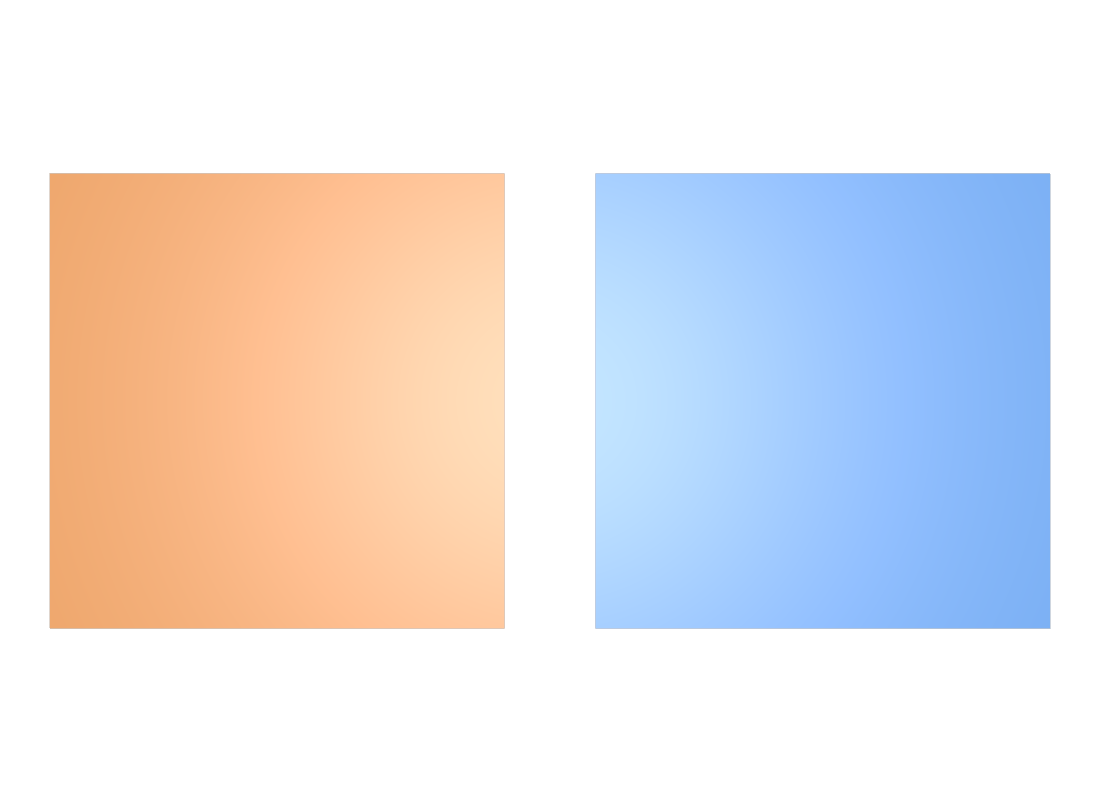
\includegraphics[width=0.88\linewidth]{figures/c17_primvar_material.png}
  \caption{The listing above rendered with \texttt{usdrecord}: both plates
  bind the \emph{same} material; the \texttt{UsdPrimvarReader} pulls each
  mesh's own \texttt{displayColor} into \texttt{diffuseColor}.}
  \label{fig:primvar-material}
\end{figure}

\begin{figure}[ht]
  \centering
  \begin{tikzpicture}[node distance=4mm and 7mm]
    \node[primbox, minimum width=2.9cm, align=center] (reader) {Reader\\ \scriptsize UsdPrimvarReader\_float3};
    \node[primbox, minimum width=2.9cm, align=center, right=of reader] (pbr) {PBR\\ \scriptsize UsdPreviewSurface};
    \node[layerbox, minimum width=2.1cm, right=of pbr] (mat) {Material};
    \node[primbox, minimum width=1.8cm, above right=6mm and -6mm of mat] (ma) {PlateA};
    \node[primbox, minimum width=1.8cm, below right=6mm and -6mm of mat] (mb) {PlateB};
    \draw[varArc] (reader) -- node[arcLabel] {result $\to$ diffuseColor} (pbr);
    \draw[varArc] (pbr) -- node[arcLabel] {surface} (mat);
    \draw[refArc] (ma.west) -- node[arcLabel] {binding} (mat.north east);
    \draw[refArc] (mb.west) -- node[arcLabel] {binding} (mat.south east);
    \node[notetext, below=2mm of reader] {varname = "displayColor"};
  \end{tikzpicture}
  \caption{The same network as a graph: connections flow left to right;
  bindings are relationships from gprims to the material.}
  \label{fig:shade-graph}
\end{figure}

\begin{ExamTip}
Why this pattern is the exam favorite: it scales. One shared material +
per-prim primvars keeps instancing intact (Content Aggregation chapter) and
avoids a material explosion --- exactly the reasoning Sample Question 10
rewards.
\end{ExamTip}

\subsection{Walking a network in code}\label{sec:vis-walk}\objref{8.2, 8.3}
Everything is prims and properties, so the network is introspectable ---
this is also how validators check shading:

\begin{lstlisting}[language=Python]
from pxr import Usd, UsdShade

stage = Usd.Stage.Open("shaded.usda")
mesh = stage.GetPrimAtPath("/Scene/PlateA")

material, rel = UsdShade.MaterialBindingAPI(mesh).ComputeBoundMaterial()
print(material.GetPath())               # /Scene/Looks/Painted

src = material.GetSurfaceOutput().GetConnectedSource()
pbr = UsdShade.Shader(src[0].GetPrim())
print(pbr.GetIdAttr().Get())            # UsdPreviewSurface

rsrc = pbr.GetInput("diffuseColor").GetConnectedSource()
reader = UsdShade.Shader(rsrc[0].GetPrim())
print(reader.GetIdAttr().Get(),         # UsdPrimvarReader_float3
      reader.GetInput("varname").Get()) # displayColor
\end{lstlisting}

\subsection{Textures, cameras, and a light}\label{sec:vis-tex}\objref{8.2, 8.4}
\index{UsdUVTexture}One node upgrades the network from flat color to
textured: \texttt{UsdUVTexture} reads an image, steered by a \texttt{float2}
primvar reader for UVs. The same scene carries a camera and a light ---
prims like everything else:

\begin{lstlisting}
#usda 1.0
( defaultPrim = "Scene" )
def Xform "Scene" {
    def Mesh "Plate" (
        prepend apiSchemas = ["MaterialBindingAPI"]
    )
    {
        int[] faceVertexCounts = [4]
        int[] faceVertexIndices = [0, 1, 2, 3]
        point3f[] points = [(-1, -1, 0), (1, -1, 0), (1, 1, 0), (-1, 1, 0)]
        texCoord2f[] primvars:st = [(0, 0), (1, 0), (1, 1), (0, 1)] (
            interpolation = "vertex"
        )
        rel material:binding = </Scene/Looks/Checkered>
    }
    def Scope "Looks" {
        def Material "Checkered" {
            token outputs:surface.connect = </Scene/Looks/Checkered/PBR.outputs:surface>
            def Shader "PBR" {
                uniform token info:id = "UsdPreviewSurface"
                color3f inputs:diffuseColor.connect = </Scene/Looks/Checkered/Tex.outputs:rgb>
                token outputs:surface
            }
            def Shader "Tex" {
                uniform token info:id = "UsdUVTexture"
                asset inputs:file = @./checker.png@
                float2 inputs:st.connect = </Scene/Looks/Checkered/Reader.outputs:result>
                color3f outputs:rgb
            }
            def Shader "Reader" {
                uniform token info:id = "UsdPrimvarReader_float2"
                string inputs:varname = "st"
                float2 outputs:result
            }
        }
    }
    def Camera "Cam" {
        float focalLength = 35
        float2 clippingRange = (0.1, 1000)
        double3 xformOp:translate = (0, 0, 6)
        uniform token[] xformOpOrder = ["xformOp:translate"]
    }
    def DistantLight "Sun" {
        float inputs:intensity = 1000
    }
}
\end{lstlisting}

\begin{figure}[ht]
  \centering
  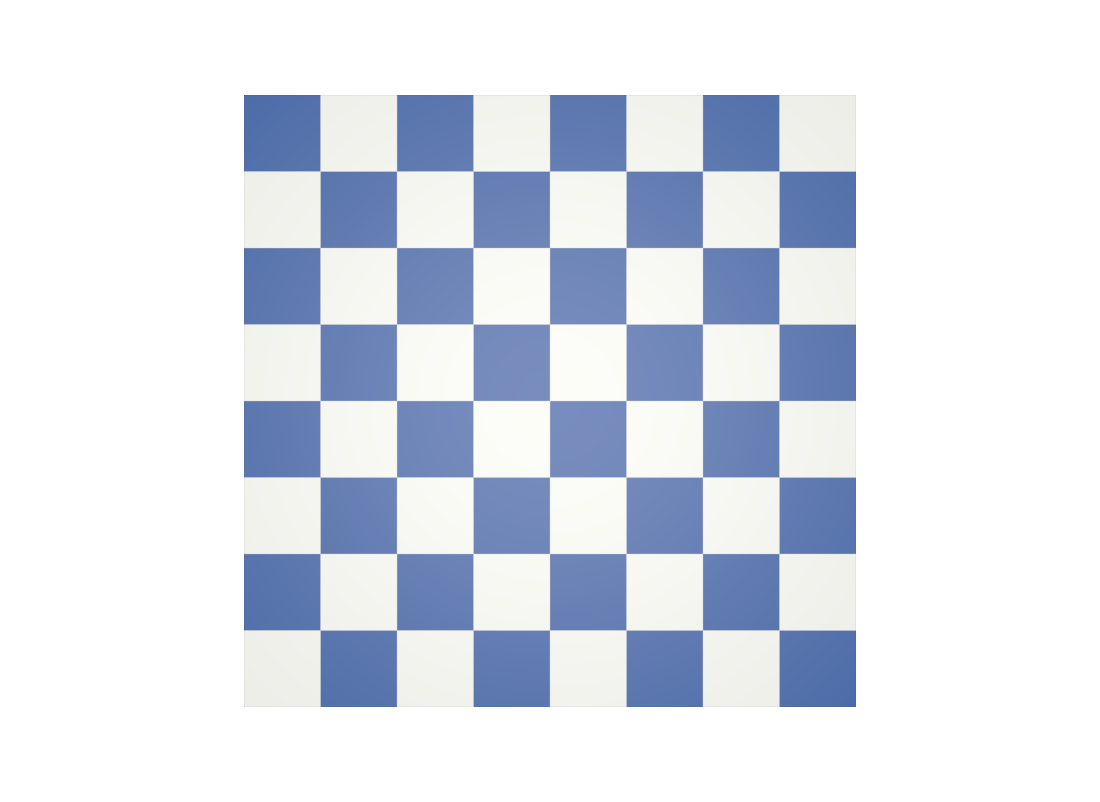
\includegraphics[width=0.8\linewidth]{figures/c17_textured.png}
  \caption{The listing rendered with \texttt{usdrecord --camera /Scene/Cam}:
  \texttt{UsdUVTexture} drives \texttt{diffuseColor}, the authored
  \texttt{DistantLight} does the lighting, the authored \texttt{Camera}
  frames the shot --- the whole render pipeline as scene description.}
  \label{fig:textured}
\end{figure}

\noindent The chain to memorize: \texttt{primvars:st} $\to$
\texttt{UsdPrimvarReader\_float2} $\to$ \texttt{UsdUVTexture.st}; the
texture's \texttt{rgb} output $\to$ \texttt{diffuseColor}. Cameras
(\texttt{UsdGeomCamera}: \texttt{focalLength}, \texttt{clippingRange},
projection) and lights complete the picture: a renderer needs nothing that
is not on the stage.\index{camera}

\subsection{Per-face materials: GeomSubset}\label{sec:vis-subset}\objref{8.3}
\index{GeomSubset}Different materials on different faces of \emph{one} mesh
--- no splitting:

\begin{lstlisting}
#usda 1.0
( defaultPrim = "Plate" )
def Mesh "Plate" (
    prepend apiSchemas = ["MaterialBindingAPI"]
)
{
    int[] faceVertexCounts = [4, 4]
    int[] faceVertexIndices = [0, 1, 2, 3, 2, 3, 4, 5]
    point3f[] points = [(-1, 0, -1), (1, 0, -1), (1, 0, 1), (-1, 0, 1),
        (1, 0, 3), (-1, 0, 3)]
    def GeomSubset "Front" {
        uniform token elementType = "face"
        int[] indices = [0]
        uniform token familyName = "materialBind"
    }
}
\end{lstlisting}

\noindent A subset names faces by index; \texttt{familyName =
"materialBind"} marks it as a binding target --- author
\texttt{material:binding} on the \emph{subset} prim exactly as on a mesh.
Subsets in a binding family should partition the faces: every face in
exactly one subset.

\begin{Gotcha}
GeomSubset relies entirely on \emph{face indices} --- change the topology
(triangulate, delete faces, re-export from a DCC) and every subset silently
points at different faces. Validate subsets after any topology-touching
step; this is a favorite ``unexpected visual result'' on round-trips.
\end{Gotcha}

\subsection{Purpose and visibility}\label{sec:vis-purpose}\objref{5.5, 6.4}
\index{purpose}\index{visibility}Two imageable controls decide what draws:

\begin{lstlisting}
#usda 1.0
( defaultPrim = "Rig" )
def Xform "Rig" {
    token visibility = "invisible"
    def Sphere "ProxySphere" {
        uniform token purpose = "proxy"
    }
    def Sphere "RenderSphere" {
        uniform token purpose = "render"
    }
}
\end{lstlisting}

\begin{lstlisting}[language=Python]
from pxr import Usd, UsdGeom

stage = Usd.Stage.Open("purpose.usda")
proxy = UsdGeom.Imageable(stage.GetPrimAtPath("/Rig/ProxySphere"))
print(proxy.ComputeVisibility())   # invisible -- inherited from /Rig
print(proxy.ComputePurpose())      # proxy
\end{lstlisting}

\noindent\texttt{visibility} (\texttt{inherited}/\texttt{invisible}) flows
down namespace --- an invisible ancestor hides the subtree.
\texttt{purpose} tags subtrees for consumers: viewports draw
\texttt{proxy}, final renders draw \texttt{render}, \texttt{guide} is for
rig helpers, and \texttt{default} draws everywhere.

\subsection{Lights are prims: UsdLux}
\index{UsdLux}Lighting follows the same schema logic as geometry and
shading. Common controls (\texttt{inputs:intensity}, \texttt{inputs:color},
\texttt{inputs:exposure}) come from \texttt{LightAPI}; light types add their
own (\texttt{DistantLight} has \texttt{inputs:angle} --- the sun's angular
size); \texttt{ShadowAPI} and \texttt{ShapingAPI} layer on shadow tinting
and IES-style shaping:

\begin{lstlisting}
#usda 1.0
( defaultPrim = "Sun" )
def DistantLight "Sun" {
    float inputs:intensity = 500
    float inputs:angle = 0.53
}
\end{lstlisting}

\begin{FieldNote}
For this domain, \texttt{usdview} is all the practice tooling you need ---
no Omniverse, no special hardware. Every render in this book was produced
with stock \texttt{usdrecord} and \texttt{usdview} on the scenes printed
beside it.
\end{FieldNote}

\DrillsTitle
\subsection*{Drill 1: Material binding}
Write a minimal example that binds a material at \texttt{/World/Looks/MyMat}
to \texttt{/World/Geo/MyMesh}.
\AnswerLines{10}
\begin{DrillSolution}
On the mesh prim: apply the schema and author the relationship ---
\texttt{prepend apiSchemas = ["MaterialBindingAPI"]} in the prim metadata,
and \texttt{rel material:binding = </World/Looks/MyMat>} in the body. In
Python: \texttt{UsdShade.MaterialBindingAPI.Apply(prim).Bind(material)}.
Verify with \texttt{ComputeBoundMaterial()} --- binding resolution respects
strength and ancestors, so trust the computed answer, not your eyes.
\end{DrillSolution}

\subsection*{Drill 2: GeomSubset use-case}
Describe when you would use GeomSubset and what data it relies on.
\AnswerLines{6}
\begin{DrillSolution}
Multiple materials on one mesh (label vs glass of a bottle) without
splitting geometry. It relies on \texttt{elementType = "face"} plus face
\emph{indices}, grouped under \texttt{familyName = "materialBind"} --- which
is why topology changes invalidate subsets.
\end{DrillSolution}

\subsection*{Drill 3: Network reading}
Without running it, predict the three printed lines of the
``walking a network'' listing, then run it mentally backwards: which edit
would make both plates render gray?
\AnswerLines{6}
\begin{DrillSolution}
It prints the material path, \texttt{UsdPreviewSurface}, and
\texttt{UsdPrimvarReader\_float3 displayColor}. Gray plates: break the chain
--- e.g.\ \texttt{varname} naming a primvar the meshes don't have (the
reader returns its fallback), or disconnecting
\texttt{inputs:diffuseColor}.
\end{DrillSolution}

\section*{Checkpoint Questions}
\addcontentsline{toc}{section}{Checkpoint Questions}

\noindent\textbf{CQ1.} One mesh must show different colors in viewport
preview vs final render. Sketch the cheapest USD-native setup.
\begin{DrillSolution}
Two sibling subtrees under the asset: a \texttt{purpose = "proxy"} version
(cheap shading) and a \texttt{purpose = "render"} version --- the renderer's
purpose selection switches; no variant or material surgery needed.
\end{DrillSolution}

\noindent\textbf{CQ2.} \texttt{ComputeBoundMaterial()} returns nothing for a
mesh that clearly has \texttt{material:binding} authored. Two likely causes?
\begin{DrillSolution}
The binding targets a prim that doesn't compose (outside
\texttt{defaultPrim} when referenced --- Sample Question 12), or the
\texttt{MaterialBindingAPI} schema isn't applied so the binding is ignored
by schema-strict consumers. Check the target's existence first.
\end{DrillSolution}

\noindent\textbf{CQ3.} Which API holds \texttt{inputs:intensity} shared by
every light type, and which API would you add for light-cone shaping?
\begin{DrillSolution}
\texttt{LightAPI} carries the shared inputs (intensity, color, exposure);
\texttt{ShapingAPI} adds cone/focus/IES controls. (\texttt{ShadowAPI} is the
third of the family --- shadow enable/color/falloff.)
\end{DrillSolution}

\subsection*{Mini-checklist (tick when mastered)}
\begin{itemize}[leftmargin=*]
  \item[$\square$] I can author the primvar-reader network from memory.
  \item[$\square$] I can walk mesh $\to$ material $\to$ shaders in Python.
  \item[$\square$] I know why GeomSubsets break on topology changes.
  \item[$\square$] I can place purpose/visibility on the right prim the first time.
\end{itemize}
